\documentclass[11pt,a4paper]{report}

\usepackage[polish]{babel}
\usepackage[utf8x]{inputenc}
\usepackage{polski}
%\usepackage[T1]{fontenc}
\frenchspacing

\usepackage{multirow}
\usepackage{indentfirst}
\usepackage{amsthm}
\usepackage{amsmath}
\usepackage{algorithmic}
\usepackage{algorithm}
\usepackage{array}
\usepackage{graphicx}
\usepackage{listings}
\usepackage{listing}
\usepackage{float}
\usepackage{colortbl}


\newtheorem{definicja}{Definicja}
\newtheorem{Observ}{Obserwacja}
\definecolor{kugray5}{RGB}{224,224,224}

\pagenumbering{arabic}

\graphicspath{{img/}}

\begin{document}
\tableofcontents
%\chapter{Wstęp [TODO]}

TODO

\chapter{Opis problemu}

Praca ma na celu zbadanie problemu wyszukiwania dokumentów w wybranym serwisie społecznościowym. Badany tutaj serwis jest zbiorem odnośników do zasobów internetowych. Każdy z nich został dodanych przez użytkowników serwisu i opisanych odpowiednimi tagami, zwanymi również etykietami. Przykładem serwisów działających w opisany tutaj sposób jest delicous czy flickr. Wynikiem pracy będzie system pozwalający na wyszukiwanie w zebranym zbiorze dokumentów, sortujący wyniki w zależności od wybranych rankingów dokumentów i prezentujący otrzymane wyniki użytkownikowi.

W pracy tej zostanie zaprezentowane kilka algorytmów wyszukujących w zbiorze dokumentów. Jako pierwsze opisane zostaną dwa algorytmy: Adapted PageRank i SocialPageRank. Algorytmy te bazują na popularnym algorytmie PageRank.  Kolejnym wykorzystanym algorytmem jest wersja algorytmu TF-IDF, który wyszukuje i porządkuje dokumenty ze względu na zapytanie i treść dokumentu. Jako dodatkowy element, zostaną użyte również dane mówiące o popularności danych wyników pozyskane z innych serwisów społecznościowych, takich jak twitter, facebook czy digg. Dane z tych stron zostały również wykorzystane w trakcie testów, do oceniania poprawności wyników.

W pracy opisane powyżej algorytmy zostaną przetestowane na zbiorze zebranych danych. Zbiór ten składa się z około 300 000 dokumentów, 200 000 użytkowników i 80 000 tagów pobranych z serwisu delicous.com. Na koniec zostanie zaprezentowany ranking łączący wszystkie zaimplementowane algorytmy. 



FOLKSONOMIA

Użytkownicy i tagi identyfikowani są na podstawie ich unikalnych nazw własnych i identyfikatorów. Dokumenty mogą być różnymi danymi: stronami www, zdjęciami, plikami np: pliki pdf. Ta praca bazuje na danych pobranych z witryny delicous, które są stronami internetowymi. Dane, które nie spełniają tego warunku, nie są brane pod uwagę w tej pracy. 

\section{Opis metod rankingu dokumentów}

Do wyliczenia rankingu dokumentów zostało użyte kilka metod. Pierwsze dwie metody to statyczne rankingi Adapted PageRank i SocialPageRank. Algorytmy te biorą pod uwagę popularność tagów, użytkowników, dokumentów i wzajemne relację między nimi. 

Kolejnym użytym w pracy rankingiem jest wersja algorytmu TF-IDF zaimplementowana we frameworku Lucene. 

Ostatnią metodą stanowiącą o popularności dokumentów są dane z serwisów takich jak facebook, twitter czy digg mówiące o ilości udostępnień danego zasobu przez użytkowników tych serwisów. 






%\documentclass[11pt,a4paper]{report}

%\usepackage[polish]{babel}
%\usepackage[utf8x]{inputenc}
%\usepackage{polski}



%\frenchspacing
%\usepackage{indentfirst}
%\usepackage{amsthm}
%\usepackage{amsmath}
%\usepackage{algorithmic}
%\usepackage{algorithm}
%\usepackage{array}
%\usepackage{multirow}
%\usepackage{graphicx}
%\usepackage{listings}
%\usepackage{float}
%\pagenumbering{arabic}

%\graphicspath{{img/}}

%\begin{document}
%\tableofcontents
\chapter{State of the art}

Obecnie prowadzonych jest wiele badań nad sieciami społecznymi używającymi etykiet (tzw. tagów, czy adnotacji) do porządkowania zasobów użytkownika. Część z nich za cel stawia sobie ulepszenie algorytmów wyszukiwania dokumentów, inne używają tych zasobów dla personalizacji wyników dla użytkowników, rekomendacji dokumentów, użytkowników, czy tagów w czasie procesu etykietowania.

Autorzy prac \cite{yanbe2007} i \cite{citeulike:3423869} analizują użyteczność etykietowania dokumentów przy wyszukiwaniu. Ich analizy bazują głównie na danych systemu delicious. Wnioski z tych prac są pozytywne. Zwracają one uwagę na korelacje miedzy popularnością stron w serwisie, a ich rankingiem według algorytmu PageRank. Dodatkowo wskazują na problemy z nowymi dokumentami dodanymi do sieci, z którymi nie radzą sobie algorytmy bazujących na odnośnikach pomiędzy dokumentami, a które mogą być rozwiązane przez strony takie jak delicous. Również rozwiązanie problemu nowych danych jest zaproponowane w pracy \cite{citeulike:8024203}. W tym artykule, jako rozwiązania, autorzy proponują użycie informacji pobranych z systemu twitter, który służącego do mikro-blogowania. Pod uwagę brane są krótkie informacje umieszczane przez użytkowników zawierające odnośniki do dokumentów jak również inne informacje dostępne w profilu użytkownika.

Autorzy pracy \cite{hotho2006information} zaprezentowali formalny model folksonomi i algorytmy AdaptedPageRank i jego bardziej spersonalizowana wersję algorytm FolkRank. Oba te algorytmy bazują na metodzie PageRank. Algorytm ten pozwala na rekomendacje tagów dla użytkowników jak również na ustalenie rankingu w wyszukiwanych elementach. 

W pracy \cite{bao2007social} przedstawione zostały algorytmy SocialSimRank i SocialPageRank. Algorytm SocialPageRank jest statycznym rankingiem zasobów, opartym również o ideę algorytmy PageRank. Algorytm ten bierze pod uwagę ilość tagów wskazujących na dany dokument jak również różną wagę opisujących dokument etykiet. Drugim proponowanym w tej pracy algorytmem jest SocialSimRank, który estymuje podobieństwo między używanymi tagami, a następnie wyniki te są używane dla wyliczanie podobieństwa między zapytaniem użytkownika a tagami przypisanymi do danego zasobu.

W pracach \cite{citeulike:3063696} i \cite{citeulike:3423905} autorzy biorą pod uwagę całą sieć społecznościową użytkownika, dodając dodatkowo znajomości użytkowników i wykorzystują te dane dla przedstawienia spersonalizowanych wyników. W artykule \cite{citeulike:3063696} opisywany jest algorytm ContextMerge, który wykonuje wyszukiwanie biorąc pod uwagę zależności między użytkownikami.  Dodatkowo pozwala na dynamiczne dodawanie nowych wyników do odpowiedzi dla uzyskania $k$. W pracy \cite{citeulike:3423905} autorzy zaproponowali system, który łączy wyniki wyszukiwarki z danymi użytkownikami aplikacji takich jak delicous. Jako bazowa wyszukiwarka może być użyta dowolna aplikacja, która zwraca dokumenty wraz z przypisanym do nich rankingiem. Wyniki te są następnie przeliczane za pomocą danych uzyskanych od użytkownika, czyli ze zbiorem dokumentów i tagów opisanych przez niego i innych użytkowników. Jako rezultat otrzymujemy nowy, bardziej spersonalizowany ranking dokumentów.

W pracy \cite{conf/mir/RawashdehKE11} celem autorów było spersonalizowanie wyników wyszukiwania w dokumentach z tagami. Do tego celu stworzone zostały dwa modele: użytkownik-tag, który ukazuje jak użytkownik użył tagi podobne do wybranego tagu. Drugim modelem jest model tag-zasób opisujący w jaki sposób dokumenty podobne do danego zasobu zostały opisane etykietami. 



Probabilistyczne podejście do rankingu dokumentów przy użyciu tagów zostało zaprezentowane w pracy \cite{citeulike:2775088} i \cite{citeulike:8846111}. W \cite{citeulike:2775088} autorzy zaprezentowali model probabilistyczny dla generowania etykiet i zależnych im dokumentów i wyszukiwania ich tematów. W \cite{citeulike:8846111} autorzy prezentują metodę rankingu tagów w zależności od ich tematu i konstruują graf przejścia między tagami należącymi do różnych tematów. Metoda ta jest wykorzystana następnie dla rekomendacji tagów dla użytkownika w czasie opisywania dokumentów. 







% [1] Web Search Personalization via Social Bookmarking and Tagging
% Michael G. Noll and Christoph Meinel
% http://data.semanticweb.org/pdfs/iswc-aswc/2007/ISWC2007_RT_Noll.pdf


% [2] can social bookmarkign enhance search in the web ?
%
% [3] can social bookmarking improve web search ?
%
% [4] time is of the essence: imprving recenct ranking using twitter data








% [7] exploring social annotations for information retrieval
% ding zhou

% [8] topic-based ranking in folksonomy via probabilistic model
% yan'an Jin

% [9] optimizing web search using social annotations

% [10] information retrieval in folksonomies: search and ranking

% [11] efficient top-k querying over Social-Tagging Networks

% [12] folksonomu-boosted social media search and ranking. 



% [5]  Exploring Folksonomy for Personalized Search  
%  http://datamining.dongguk.ac.kr/work/project/KDI/CVM/%EC%B5%9C%EC%A2%85%ED%99%94%EC%9D%BC-1.%EA%B2%BD%EB%82%A8%EB%A1%9C%EB%B4%87%EB%9E%9C%EB%93%9C%281%EC%B0%A8%EC%A1%B0%EC%82%AC%29/p155-xu-Exploring%20folksonomy%20for%20personalized%20search%20.pdf 


% [6] Personalization of Tagging Systems
% http://ict.ewi.tudelft.nl/pub/jun/ptIPM.pdf

% W mojej pracy skupie się na dwóch algorytmach: adapted pagerank i socialpagerank. Postaram się porownać wyniki działania tych dwóch algorytmów jak również zaproponuje użycie innych danych z innych serwisów społecznościowych takich jak twitter, facebook i digg do poprawienia jakości wyszukiwanych materiałów.






%\bibliographystyle{plain}
%\bibliography{biblio}


%\end{document}


\chapter{Algorytmy}


\section{Folksonomia}

Folksonomią nazywamy społeczne klasyfikowanie, czy tagowanie różnych zasobów. Formalnie model folksonomii został przedstawiony w pracy \cite{hotho2006information}. Można ja przedstawić jako krotkę $F := (U,T,R,Y)$, gdzie:
$U$,$T$,$R$ to zbiory skończone, których elementy składają się odpowiednio z użytkowników, tagów i dokumentów. $Y$ jest relacją “przypisania tagu” pomiędzy tymi elementami $Y \subseteq U \times T \times R$

Użytkownicy i tagi identyfikowani są na podstawie ich unikalnych nazw własnych. Dokumenty mogą być różnymi danymi: stronami www, zdjęciami, plikami np: pliki pdf. Ta praca bazuje na danych pobranych z witryny delicous, które w zdecydowanej większości są stronami www. Dane które nie są stroną www nie są brane pod uwagę w tej pracy. 





\chapter{SocialPageRank}
\section{Opis}
SocialPageRank jest statycznym rankingiem stron z perspektywy użytkownika sieci. Algorytm bazuje na obserwacji relacji miedzy popularnymi stronami, tagami i udzielającymi sie użytkownikami. Popularne strony są dodawane przez udzielających się użytkowników, które są opisywane popularnymi tagami. Udzielający się użytkownicy używają popularnych tagów dla popularnych stron. Popularne tagi używane są do annotacji popularnych stron przez ważnych użytkowników.

Bazując na powyższych założeniach algorytm propaguje i wzmacnia zależności między popularnymi tagami, użytkownikami i dokumentami. 
\subsection*{Dane wejsciowe:}
$N_T$: ilośc tagów

$N_U$: ilośc użytkowników

$N_D$: ilośc dokumentów

$M_{DU}$: macierz $N_D \times N_D$ asocjacyjna między dokumentami a użytkownikami

$M_{UT}$: macierz $N_U \times N_T$  asocjacyjna między użytkownikami a tagami

$M_{TD}$: macierz $N_T \times N_D$ asocjacyjna między tagami a dokumentami

$P_0$: wektor, od długości $N_D$, 

\subsection*{Inicjalizacja}
W komórce macierzy$M_{DU}(d_n, u_k)$ znajduje się wartość będąca ilością annotacji przypisanych do dokumentu $d_n$ przez użytkownika $u_k$. Podobnie dla pozostałych macierzy, elementy $M_{UT}(u_k, t_n)$ to ilość dokumentów opisanych tagiem $t_n$ przez użytkownika $u_k$, elementy$M_{TD}(t_n, d_k)$: ile użytkowników dodawało dokument $d_k$ i oznaczyło go annotacją $t_n$. 

Wektor $P_0$ zainicializowany został losowymi wartościami z przedziału $[0,1]$. Jest on pierwszym przybliżeniem rank dokumentów.


\begin{algorithmic}
\REPEAT
\STATE $U_i = M_{DU}^T * P_i$
\STATE $T_i = M_{UT}^T * U_i$
\STATE $P_i’ = M_{TD}^T * T_i$
\STATE $T_i’ = M_{TD}  * P_i’$
\STATE $U_i’ = M_{UT} * T_i’$
\STATE $P_(i+1) = M_{DU} * U_i’$
\UNTIL{ wartości wektora $P_n$ nie zbiegną }
\end{algorithmic}

\subsection*{Złożność}
Złożoność czasowa każdej iteracji wynosi $O(N_u*N_d + N_t*N_d + N_t*N_u)$.

\section{Wyniki algorytmu dla przykładowych danych}

W poniższej tabelce znajdują sie dane, dla których zostało sprawdzone działanie algorytmu Social PageRank. Dane są nie duże i składają sie z trzech różnych dokumentów, dwóch użytkowników i trzech tagów.

\renewcommand{\multirowsetup}{\centering}
\begin{center}
\begin{tabular}{|l| r | r| }
\hline
\multirow{3}{5cm}{\centering Strony www}
& \multicolumn{2}{p{6cm}|}%
{\centering użytkownicy}\\
\cline{2-3}
& \multicolumn{1}{c|}{użytkownik 1}
& \multicolumn{1}{c|}{użytkownik 2}\\
\hline
http://www.ted.com/ & inspiration & \\
http://www.colourlovers.com/&	design & inspiration \\
http://www.behance.net/	&portfolio, design & portfolio, inspiration \\
\hline
\end{tabular}
\end{center}

Dla takich danych macierz $M_{d,u}$ mówiąca o zależności dokumentów z użytkownikami ma postać:

\[
 M_{d,u} =
 \begin{pmatrix}
  1 & 0 \\
  1 & 1 \\
  1 & 2
 \end{pmatrix}
\]

Maciez użytkowników i tagów, $M_{u,t}$:

\[
 M_{u,t} =
 \begin{pmatrix}
  1 & 1 & 1 \\
  2 & 0 & 1 
 \end{pmatrix}
\]

Maciez tagów i dokumentów, $M_{t,d}$:
\[
 M_{t,d} =
 \begin{pmatrix}
  1 & 1 & 1 \\
  0 & 1 & 1 \\
  0 & 0 & 2 
 \end{pmatrix}
\]


\subsection*{wyniki:}
Dla powyższych danych wyniki algorytmu zbiegają po czterech iteracjach z dokładnościa
$|P_3 - P_4|  < 10^{-10}$. Wyniki zostały przedstawione w poniższej tabelce:

\begin{tabular}{|l|r|}
\hline
\multicolumn{1}{|m{4.5cm}|}{  }
&\multicolumn{1}{m{5.3cm}|}%
{\centering Social PageRank }\\
\hline
www.ted.com & 0.2381373691295440 \\
www.colourlovers.com  & 0.4343479235414989 \\
www.behance.net & 0.8686958470829979 \\
\hline
\end{tabular}


Można zauwazyć, że największy ranking ma strona behance.net ktora została dodana przez dwóch użytkowników i oznaczonych najpopularniejszymi tagami - 2 razy tagiem portfolio, użytym tylko dla tej strony, raz tagiem design, który użyty był 2 razy w powyższych danych i również raz tagiem inspiration, który jest najpopularniejszym tagiem, użytym w przykładzie aż 3 razy. 

\section{Implementacja}

Algorytm pozwala na wczesniejsze wyliczenie rankingu dlatego został zaimplementowany jako osobny proces działający działający w określonych okresach czasu. Dodatkowo algorytm wymaga danych, które muszą być wyliczone i zapisane w bazie danych przed rozpoczęciem jego działania.  

\subsection{Baza danych}
Poniżej znajduje się obrazek przestawiający bazę danych ze zmianami wymaganymi dla sprawnego działania algorytmu. Dodatkowe tabele dodane zostały dla przyśpieszenia generowania danych wejściowych. Dane w nich zawarte wyliczane są z danych wyliczane są z danych już istniejących w bazie danych.



TODO: OBRAZEK - BAZA DANYCH Z DODATKOWYMI TABELAMI I ZAZNACZONYMI UZYWANYMI POLAMI W BAZIE DANYCH


Tabela DOKUMENT zawiera dodatkowo pole soc\_page\_rank służące do przechowywania wyników algorytmu. Tabele TAG\_USR i TAG\_DOC jak równiez pole w tabeli USERTAGDOC.how\_much zawieraja redundantne dane wykorzystywane do generowania macierzy. Pole USERTAGDOC.how\_much zawiera informacje o ilości tagów użytych przez użytkownika do opisania dokumentu. TAG\_USR zaiera relacje miedzy użytkownikami i tagami, ilość annotowanych dokumentów przez tą parę znajduje się w polu how\_much. Analogicznie TAG\_DOC jest relacja między annotacjami a dokumentami z ilością ich wykorzystania.

\subsection{Tworzenie i mnożenie macierzy}

Algorytm wymaga w każdej iteracji wykorzystania sześć macierzy. Z powodu wielkości danych nie jesteśmy w stanie przechowywać ich wszystkich w pamięci. Dodatkowo biblioteka wykorzystana do mnożenia macierzy nakłada ograniczenia na ilość kolumn i wierszy w macierzach. Kolejnym problemem jest czas potrzebny na pobranie danych z bazy danych.

Z powodu tych ograniczeń macierze pobierane są do partiami do pamięci z bazy danych, przetwarzane i zapisywane są w struktury ułatwiające szybki do nich dostęp. Następnie, zapisywane są w plikach zawierające największe porcje danych mieszczące się jednocześnie w pamięci.

W każdej iteracji algorytm pobiera dane z dysku. Z tych danych tworzona jest macierz o maksymalnej możliwej ilości wierszy na które pozwala wykorzystana biblioteka. Każda z tych częsci jest osobno mnożona przez wektor. Wyniki następnie składane są w wektorze wynikowym, który przekazywany jest do kolejnego mnożenia macierzy

WYKRES POKAZUJACY PROCES TWORZENIA I MNOZENIA CZĘŚCIOWEGO MACIERZY



Mimo, że wymagania pamięciowe sprawiają, że trzeba wykonać wiekszą liczbe działań w czasie mnożenia, macierze generowane są dość rzadkie. Wiekszość pól zawiera wartość 0, co przyśpiesza mnożenie macierzy i wektorów.

TODO: ilosc wykorzystanych plików przy prawdziwych danych (1 mln)

TODO: ilość mnożen 

TODO: wykorzystana biblioteka: cern.colt


\section{Wyniki - czesciowe: TODO}

// wyniki dla danych 66 000 dokumentów - TODO - wyniki dla duzych danych

Strona http://www.pythonchallenge.com/ jest jedną ze stron z najwiekszym wynikiem socialpagerank ( 0.00301). Dodane jest przez 785 różnych użytkowników. Zostało użyte do tego 209 unikalnych tagów. Najpopularniesze tagi, w kolejności od najczęsciej użytego to python, programming, challage i puzzle.

jedną ze stron o najnizszym rankingu jest np: http://djangosnippets.org/snippets/1314/ . Strona ta zawiera specificzne rozszerzenie dla frameworku django. Można sie spodziewać ze nie bedzie to popularna witryna. Została ona dodana przez jednego użytkownika i opisana siedmioma annotcjami.

Strony które uzyskały ranking 0 to strony które nie zostały opisane zadnymi tagami przez użytkowników. 

\subsection{Problemy : TODO}
Potencjalne problemy zauwazone na mniejszej ilości danych: algorytm jest podatny na cykle które mogą zostać stworzone przez dużą ilość wygenerowanch użytkowników.

\subsection{Przykładowe wyniki wyszukiwarki : TODO} 

TODO: OPISAC POZNIEJ, PO ZAIMPLEMENTOWANIU WYSZUKIWANIA UZYWAJACEGO SOCIALPAGERANK 













\chapter{Adapted PageRank}



\section{Lucene}


Lucene jest biblioteką napisaną w Javie. Biblioteka ta jest w stanie indeksować dużą ilość dokumentów z różnych źródeł i przeprowadzać szybkie wyszukiwania w tych tekstach. W opisywanej aplikacji, framework Lucene przechowuje źródła stron. Strony te zostały pobrane z  serwisu delicous i zapisane w bazie danych. 

\subsection{Pobieranie stron}

W pewnych odstępach czasu, wątek odpowiedzialny za indeksowanie stron sprawdza czy w bazie danych tabela DOCUMENT nie ma informacji o nowych wpisach. Z bazy danych pobrane są informacje o adresach tych stron. Następnie dla każdego adresu URL zostaje pobrana treść strony na którą wskazuje. Strona WWW następnie zostaje oczyszczona ze znaczników HTML, i przekazane do frameworku lucene do zindeksowania. Jeśli wszystkie czynności zakończą się powodzeniem, w bazie danych zostaje odnotowana informacja o posiadaniu na dysku danego dokumentu. Rysunek \ref{fig:lucene_index_fig} przedstawiony jest cały proces pobierania i przetwarzania danej strony.

\begin{figure}[htb]

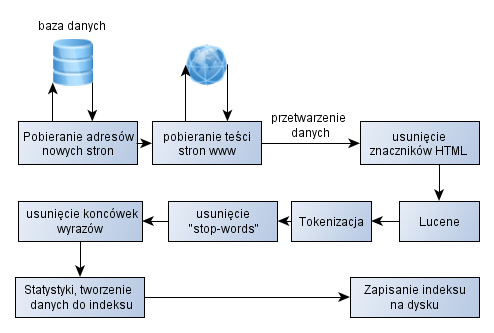
\includegraphics[width=1\textwidth]{lucene_indeksing.png}
\caption{Lucene: pobieranie danych i indeksowanie}
\label{fig:lucene_index_fig}
\end{figure}

Do Lucene zapisywane są następujące informacje: identyfikator $id$ dokumentu z bazy danych, oraz przetworzony tekst strony WWW. Przechowywanie identyfikatora dokumentu w danych Lucene pozwala późniejsze powiązanie wyników wyszukiwania z odpowiednim rekordem w bazie danych. 

W czasie indeksowania biblioteka Lucene wykonuje wiele czynności które pozwalają jej później szybko wyszukiwać informację. Główne z nich to:
\begin{itemize}
\item Tekst zostanie przetworzony na ciąg termów,
\item usunięcie końcówek wyrazów,
\item usunięcie 'stop-words' z tekstu, czyli słów nie mających dużego znaczenia przy wynikach wyszukiwania, takich jak: i, lub, ...
\item obliczenie statystyk, np: wystąpienia słów w dokumencie, odległości od siebie
\end{itemize}


Czas wyszukiwania zapytania w dokumentach przechowywanych Lucene jest szybkie. Przy małej, poniżej 1GB danych, wyszukiwanie następuje praktycznie w czasie rzeczywistym. Zapytanie jest przekazywane do frameworku, w którym jest one przekształcane na termy. Dla zapytania $q$ i dla każdego dokumentu $d$ wyliczana jest wartość funkcji $score(q,d)$. Wynikiem są dokumenty posortowane wg. wyniku tej funkcji.

$score(q,d) =   coord(q,d)  *  queryNorm(q) * \sum_{t \text{ in } q}  \bigg( tf(t\text{ in } d)  *  idf(t)^2  *  getBoost(t) *  norm(t,d) )$

gdzie:
\begin{itemize}
	\item coord(q,d): funkcja zwraca wartości zależne od miejsca występowania i odległości od siebie szukanych termów w dokumencie.
	\item queryNorm(q): funkcja normalizująca wyniki zapytania
	\item tf(t in d): funkcja wyliczająca częstość występowania danego termu w dokumencie
	\item idf(t) : funkcja wyliczająca częstość występowania termu we wszystkich dokumentach.
	\item getBoost(t) - Lucene pozwala na zwiększenie wagi niektórych termów. Nieużywane w tej aplikacji.
\end{itemize}

Lucene ocenia dokumenty głównie na podstawie funkcji TF-IDF. Każdy dokument reprezentowany jest przez wektor, składający się z wag słów występujących w tym dokumencie. TFIDF informuje o częstości wystąpienia termów uwzględniając jednocześnie odpowiednie wyważenie znaczenia lokalnego termu i jego znaczenia w kontekście pełnej kolekcji dokumentów.

\section{Inne rankingi}

Rankin używający danych z digg'a, twittera i facebooka
Propozycja rankingu (prosta):

\begin{itemize}
\item $d_i$ - ilość użytkowników udostepniających dokument $i$ w serwisie digg
\item $f_i$ - ilośc użytkowników udostępniających dokument $i$ w serwisie facebook
\item  $t_i$ - ilość użytkowników udostępniających dokument $i$ w serwisie twitter
\item $rank_i$ - ranking dokumentu $i$
\end{itemize}

powyższe wartości zostały znormalizowane.

$rank_i = d_i + f_i + t_i$



%\chapter{Opis aplikacji [TODO]}

\section{Folksonomia}

Folksonomia nazywamy krotkę $F := (U,T,R,Y)$, gdzie:
$U$,$T$,$R$ to zbiory skończone, których elementy składają się odpowiednio z użytkowników, tagów i dokumentów. $Y$ jest relacją “przypisania tagu” pomiędzy tymi elementami $Y < U \times T \times R$

Użytkownicy i tagi identyfikowani są na podstawie ich unikalnych nazw własnych. Dokumenty mogą być różnymi danymi: stronami www, zdjęciami, plikami np: pliki pdf. Ta praca bazuje na danych pobranych z systemu delicous, które w zdecydowanej większości są stronami www. Dane które nie są stroną www nie są brane pod uwagę w tej pracy. 

\section{Architektura}

\subsection{Zbieranie danych:}

Dane pobierane są na kilka sposobów. Głównym źródłem nowych danych jest kanał RSS strony delicous. Dodatkowo dla użytkowników i dokumentów które są już zapisane w bazie danych, co powien przedział czasu, sprawdzane jest czy nie zostały dla nich dodane nowe wpisy na stronie delicous.

\subsection*{Nowe dane}
Kanał RSS delicous zawiera dane ostatnio dodane przez użytkowników serwisu delicous. Nie są to tylko nowe dane, mogą byc to dane które istnieją na stronie, ale zostały dodane ponownie przez innego użytkownika. Każdy wpis zawiera informacje o użytkowniku który ostatnio dodał daną strone, tagi, adres strony i adres kanału rss tej strony. 


\begin{enumerate}
\item Crawler Delicous:

\begin{itemize}
\item sprawedza najnowsze dane dodawane przez wsyzstkich uzytwkoników na głównej stronie delicous.
\item sprwadza popularne strony dodawane przez uzytwkoników. To czy dana strona znajdywała sie wśród popularnych jest równiez zapusywanie w bazie danych.
\item update: sprwadzanie danych ze strony uzywtkoników którzy już są dodani jak również sprawdzanie czy strony ktore juz były dodane nie otrzymały nowych tagów i czy nie było innych uzytkowników którzy dana strone dodali równiez (pozwala to na szybkie zwiekszenie danych, ale rowniez moze spowodowac potencjalne problemy: moze to spowodowac ze dane ktore beda w bazie bedą do siebie podobne - ci sami uzytwkonicy dodaja podobne strony, w podobnej tematyce, z drugiej strony,  osoby ktorzy dodali dana strone, mogą mieć podobne preferencje)
\end{itemize}

Najnowsze dane pochodzą z przeglądania głownego RSS’a strony. Po sparsowaniu danych, wyciagane sa nowe strony. Kazdy z tych nowych URL’i posiada swoja strone na delicous, na ktorej przechowywane sa dane o uzytkownikach ktorzy dodali i tagach uzytych. Przegladane zostaje



\item Crawlery innych serwisów społecznościowych:

w swoim systemie korzystam z serwisów tweeter, facebook, digg. Dostarczaja one API ktore pozwala sprwadzic ile uzytkwoników udosteponiło dana strone. Działaja one niezaleznie od siebie. Sprawdzane są jednoczesnie nowo dodane do systemu strony jak również przeprowadzany jest update pozostałych

\item Lucene:

Zadaniem tego crawlera jest sprazanie nowo dodanych stron do systemu, i sciagniecie ich treści na dysk. Po ściagnieciu danej strony, usuwane są zniej wszystkie znaczniki HTML, a nastepnie zapisywane są na dysku przy pomocu framworku lucene.

\item cache:

\begin{itemize} 
\item statystyki -- co powiem okreslony czas na bazie danych robiony jest update statystyk. Wyliczanie statystyki powoduja jednak duze obciazenie bazy danych. Najwiekszym problemem nie jest obciazenie ale
obencie wyliczane statystyki:
\begin{itemize} 
    \item  dla uzytkownika:
	\begin{itemize} 
          		\item  ilosc dodanych dokumento
	          	\item ilość uzywanych tagów,
	          	\item najczesciej uzywane tagi
	\end{itemize}
    \item  dla dokumentu:
	\begin{itemize} 
	          	\item ile razy dodany przez uzytkowników
	          	\item ile razy został otagowany
	          	\item ile razy został otagowany rozymi słowami
	          	\item najczęstrze tagi uzywane do opisania tego dokuemtnu
	\end{itemize}
    \item  dla tagów
	\begin{itemize} 
	          \item  ile razy uzywany przez roznych uzytwkoników
	          \item  ile razy uzywany w ogóle.
	          \item  na ilu roznych dokumentach zostal uzyty
	          \item  najczestrze dokuemtny opisane tym tagiem
	          \item  uzytkownicy, uzywajacy najczesciej jego
	\end{itemize}
\end{itemize}


\end{itemize}

\item cache wyszukiwarki: w tabeli documents dodawane są rowniez dodatkowe informacje ktore są wypisywane w momencie kiedy wyszukiwarka zwroci wynik, a ich wyliczanie w czasie podawania wyniku dla uzytkownika bylo by zbyt czasochłonne. Tymi dodatkowymi rzeczami są: czesto uzywane tagi, ilość uzytkowników ktory dany tag dodała. Dane te są odrazu sformatowane i gotowe do wypisane w przeglądarce

\end{enumerate}

\subsection*{baza danych:}
jako serwer uzywany jest MySQL 5.1

komunikacja miedzy aplikacja a baza danych odbywa sie za pomocą frameworku Hibernate. Framework ten zapewnia translacje danych z relacyjnej bazy danych na obiekty używane w aplikacji.


\subsection*{front-end:}
interface uzytwkonika napisany jest przy pomocy technologi google-web-toolkit.
głowny panel zawiera u góry zakładki, które pozwalaja na przemieszczenie sie miedzy wyszukiwarką, statystykami, tagami, innymi informacjami.

uzytkownik po wczytaniu zapytaniu i nacisnieciu ENTER otrzymuje wyniki zapytania.


\subsection*{Tagi:}
Tagi nie są dodawane do bazy danych w postaci dokladnie uzyskanej ze strony delicous. Wiele z nich wymaga paru przekształcen. Podstawowym jest usuniecie białych znaków z początku i konca słowa. Dodawkowo, wiekszość tagów, zaczyna lub kończy się na znakach specjalnych, lub znajduje sie w cudzysłowiu czy też kończy się znakiem przecinka. Dla przykładu:

\begin{itemize} 
    \item @java
    \item  @@java
    \item  \#java
    \item  java@
    \item  “tag” / “tag / tag”
    \item  tekst, / ,tekst
\end{itemize}




\chapter{Implementacja}

\chapter{Opis aplikacji [TODO]}

\section{Folksonomia}

Folksonomia nazywamy krotkę $F := (U,T,R,Y)$, gdzie:
$U$,$T$,$R$ to zbiory skończone, których elementy składają się odpowiednio z użytkowników, tagów i dokumentów. $Y$ jest relacją “przypisania tagu” pomiędzy tymi elementami $Y < U \times T \times R$

Użytkownicy i tagi identyfikowani są na podstawie ich unikalnych nazw własnych. Dokumenty mogą być różnymi danymi: stronami www, zdjęciami, plikami np: pliki pdf. Ta praca bazuje na danych pobranych z systemu delicous, które w zdecydowanej większości są stronami www. Dane które nie są stroną www nie są brane pod uwagę w tej pracy. 

\section{Architektura}

\subsection{Zbieranie danych:}

Dane pobierane są na kilka sposobów. Głównym źródłem nowych danych jest kanał RSS strony delicous. Dodatkowo dla użytkowników i dokumentów które są już zapisane w bazie danych, co powien przedział czasu, sprawdzane jest czy nie zostały dla nich dodane nowe wpisy na stronie delicous.

\subsection*{Nowe dane}
Kanał RSS delicous zawiera dane ostatnio dodane przez użytkowników serwisu delicous. Nie są to tylko nowe dane, mogą byc to dane które istnieją na stronie, ale zostały dodane ponownie przez innego użytkownika. Każdy wpis zawiera informacje o użytkowniku który ostatnio dodał daną strone, tagi, adres strony i adres kanału rss tej strony. 


\begin{enumerate}
\item Crawler Delicous:

\begin{itemize}
\item sprawedza najnowsze dane dodawane przez wsyzstkich uzytwkoników na głównej stronie delicous.
\item sprwadza popularne strony dodawane przez uzytwkoników. To czy dana strona znajdywała sie wśród popularnych jest równiez zapusywanie w bazie danych.
\item update: sprwadzanie danych ze strony uzywtkoników którzy już są dodani jak również sprawdzanie czy strony ktore juz były dodane nie otrzymały nowych tagów i czy nie było innych uzytkowników którzy dana strone dodali równiez (pozwala to na szybkie zwiekszenie danych, ale rowniez moze spowodowac potencjalne problemy: moze to spowodowac ze dane ktore beda w bazie bedą do siebie podobne - ci sami uzytwkonicy dodaja podobne strony, w podobnej tematyce, z drugiej strony,  osoby ktorzy dodali dana strone, mogą mieć podobne preferencje)
\end{itemize}

Najnowsze dane pochodzą z przeglądania głownego RSS’a strony. Po sparsowaniu danych, wyciagane sa nowe strony. Kazdy z tych nowych URL’i posiada swoja strone na delicous, na ktorej przechowywane sa dane o uzytkownikach ktorzy dodali i tagach uzytych. Przegladane zostaje



\item Crawlery innych serwisów społecznościowych:

w swoim systemie korzystam z serwisów tweeter, facebook, digg. Dostarczaja one API ktore pozwala sprwadzic ile uzytkwoników udosteponiło dana strone. Działaja one niezaleznie od siebie. Sprawdzane są jednoczesnie nowo dodane do systemu strony jak również przeprowadzany jest update pozostałych

\item Lucene:

Zadaniem tego crawlera jest sprazanie nowo dodanych stron do systemu, i sciagniecie ich treści na dysk. Po ściagnieciu danej strony, usuwane są zniej wszystkie znaczniki HTML, a nastepnie zapisywane są na dysku przy pomocu framworku lucene.

\item cache:

\begin{itemize} 
\item statystyki -- co powiem okreslony czas na bazie danych robiony jest update statystyk. Wyliczanie statystyki powoduja jednak duze obciazenie bazy danych. Najwiekszym problemem nie jest obciazenie ale
obencie wyliczane statystyki:
\begin{itemize} 
    \item  dla uzytkownika:
	\begin{itemize} 
          		\item  ilosc dodanych dokumento
	          	\item ilość uzywanych tagów,
	          	\item najczesciej uzywane tagi
	\end{itemize}
    \item  dla dokumentu:
	\begin{itemize} 
	          	\item ile razy dodany przez uzytkowników
	          	\item ile razy został otagowany
	          	\item ile razy został otagowany rozymi słowami
	          	\item najczęstrze tagi uzywane do opisania tego dokuemtnu
	\end{itemize}
    \item  dla tagów
	\begin{itemize} 
	          \item  ile razy uzywany przez roznych uzytwkoników
	          \item  ile razy uzywany w ogóle.
	          \item  na ilu roznych dokumentach zostal uzyty
	          \item  najczestrze dokuemtny opisane tym tagiem
	          \item  uzytkownicy, uzywajacy najczesciej jego
	\end{itemize}
\end{itemize}


\end{itemize}

\item cache wyszukiwarki: w tabeli documents dodawane są rowniez dodatkowe informacje ktore są wypisywane w momencie kiedy wyszukiwarka zwroci wynik, a ich wyliczanie w czasie podawania wyniku dla uzytkownika bylo by zbyt czasochłonne. Tymi dodatkowymi rzeczami są: czesto uzywane tagi, ilość uzytkowników ktory dany tag dodała. Dane te są odrazu sformatowane i gotowe do wypisane w przeglądarce

\end{enumerate}

\subsection*{baza danych:}
jako serwer uzywany jest MySQL 5.1

komunikacja miedzy aplikacja a baza danych odbywa sie za pomocą frameworku Hibernate. Framework ten zapewnia translacje danych z relacyjnej bazy danych na obiekty używane w aplikacji.


\subsection*{front-end:}
interface uzytwkonika napisany jest przy pomocy technologi google-web-toolkit.
głowny panel zawiera u góry zakładki, które pozwalaja na przemieszczenie sie miedzy wyszukiwarką, statystykami, tagami, innymi informacjami.

uzytkownik po wczytaniu zapytaniu i nacisnieciu ENTER otrzymuje wyniki zapytania.


\subsection*{Tagi:}
Tagi nie są dodawane do bazy danych w postaci dokladnie uzyskanej ze strony delicous. Wiele z nich wymaga paru przekształcen. Podstawowym jest usuniecie białych znaków z początku i konca słowa. Dodawkowo, wiekszość tagów, zaczyna lub kończy się na znakach specjalnych, lub znajduje sie w cudzysłowiu czy też kończy się znakiem przecinka. Dla przykładu:

\begin{itemize} 
    \item @java
    \item  @@java
    \item  \#java
    \item  java@
    \item  “tag” / “tag / tag”
    \item  tekst, / ,tekst
\end{itemize}





\documentclass[11pt,a4paper]{report}

\usepackage[polish]{babel}
\usepackage[utf8x]{inputenc}
\usepackage{polski}
%\usepackage[T1]{fontenc}
\frenchspacing
\usepackage{indentfirst}
\usepackage{amsthm}
\usepackage{amsmath}
\usepackage{algorithmic}
\usepackage{algorithm}
\usepackage{array}
\usepackage{multirow}
\usepackage{graphicx}
\usepackage{listings}
\usepackage{float}
\pagenumbering{arabic}

\graphicspath{{img/}}

\begin{document}
\tableofcontents


\chapter{Baza danych}

\section{System zarządzania baza danych}

Jako serwer bazy danych został użyty MySQL serwer z silnikiem bazy danych InnoDB. MySQL został wybrany głównie z powodu swojej szybkości działania i z powodu prostoty używania. Dodatkowe funkcjonalności bazy danych rozbudowane w innych serwerach takich jak: PostgreSQL i Oracle, czyli funkcje, triggery, nie są używane w tej aplikacji. 

\section{Tabele}


\begin{figure}[htb]
\centering
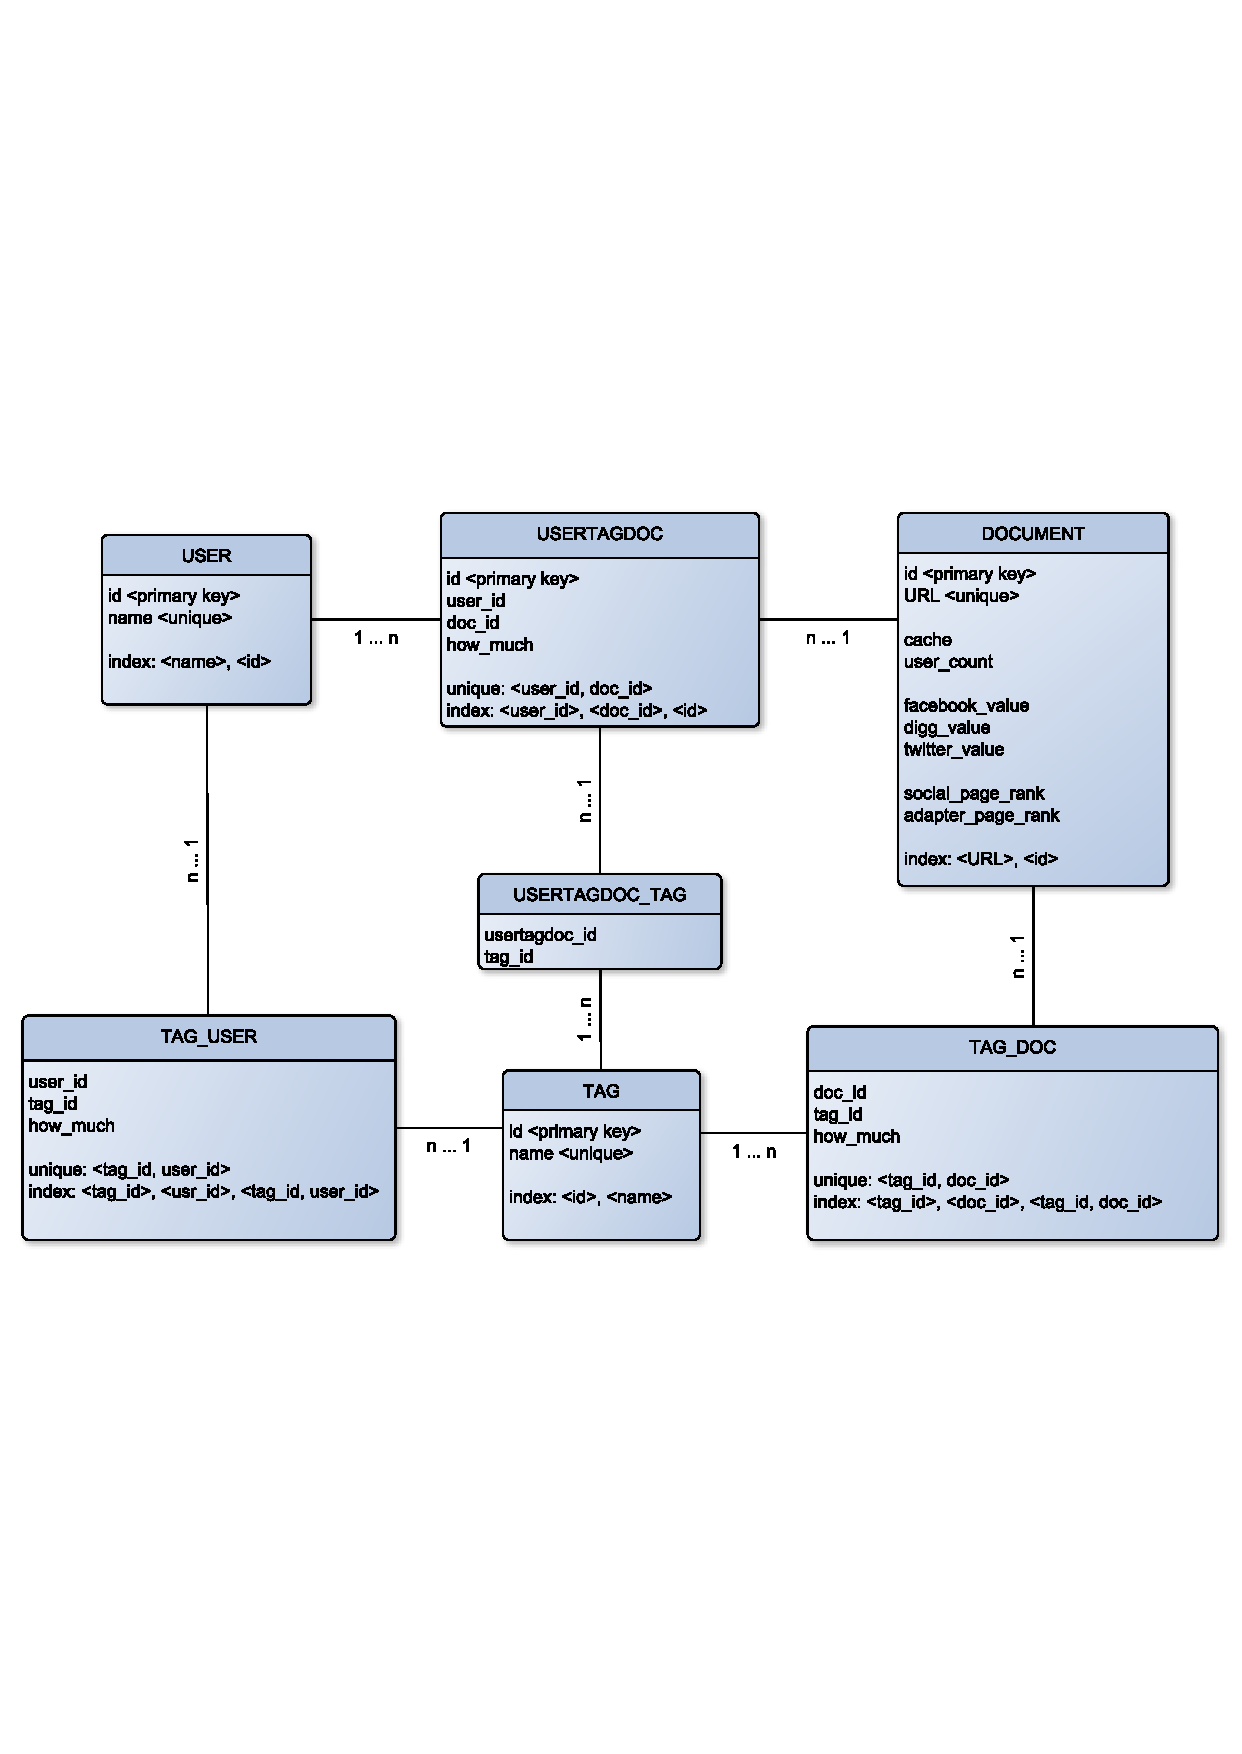
\includegraphics[width=1\textwidth]{database.pdf}
\caption{Schemat bazy danych}
\label{fig:db_fig}
\end{figure}

Baza danych składa się z trzech głównych tabel: User, Document i Tag. Zawierają one informację na temat użytkowników, dokumentów i adnotacji pobrane z serwisu delicous. W bazie danych znajdują sie też tabele: UserTagDoc i UserTagDoc\_tag, które służą do zapisania relacji między użytkownikami a dokumentami (usertagdoc) i adnotacjami (UserTagDoc\_tag). W tych tabelach zapisane są  informacje na temat tego czy dany użytkownik dodał dokument do serwisu i jakimi tagami została dana strona opisana.








\subsection{Tabele i pola pomocnicze}
Dodatkowo w bazie danych znajdują się dwie tabele: tag\_doc i tag\_user. Tabele tych zapisywane są dane wyliczone z pozostałych tabel. W tabeli tag\_doc znajdują się informację na temat tego ile razy przez różnych użytkowników dany dokument doc\_i  został dodany i opisany tagiem tag\_k. Odpowiednia w tabeli tag\_user znajdują się informację na temat ilości różnych dokumentów dodanych przez użytkownika usr\_n i opisanych tagiem tag\_m. Dane ilości różnych tagów którymi użytkownik usr\_l opisał dokument doc\_j przechowywane są w już istniejącej tabeli UserTagDoc.

Schemat bazy danych z zaznaczonymi nowymi tabelami i polem count w usertagdoc

W tabelach na różnych polach zostały dodane indeksy. Przyśpieszają one działanie aplikacji, pozwalają na szybsze operacja przy często używanych polach.
\subsection{Listing}
Poniżej znajduje się listing zapytania SQL tworzącego tabele w bazie danych.

\lstset{language=SQL}  
\begin{lstlisting}[frame=lines, caption={Skrypt tworzący tabele w bazie danych}, label={sql_all}] ]


CREATE TABLE `DOCUMENT` (
 `id` bigint(20) NOT NULL AUTO_INCREMENT,
 `url` varchar(255) NOT NULL,
 `digg_value` int(11) DEFAULT '0',
 `facebook_value` int(11) DEFAULT '0',
 `twitter_value` int(11) DEFAULT '0',
 `page_fetch` tinyint(1) DEFAULT '0',
 `tag_count` bigint(20) DEFAULT NULL,
 `user_count` bigint(20) DEFAULT NULL,
 `cache` text,
 `adapted_page_rank` double DEFAULT NULL,
 `social_page_rank` double DEFAULT NULL,
 PRIMARY KEY (`id`),
 UNIQUE KEY `url` (`url`)
) 

CREATE TABLE `TAG` (
 `id` bigint(20) NOT NULL AUTO_INCREMENT,
 `doc_count` bigint(20) DEFAULT NULL,
 `doc_dist_count` bigint(20) DEFAULT NULL,
 `tag` varchar(255) NOT NULL,
 `user_count` bigint(20) DEFAULT NULL,
 `adapted_page_rank` double DEFAULT NULL,
 PRIMARY KEY (`id`),
 UNIQUE KEY `tag` (`tag`)
)

CREATE TABLE `TAG_DOC` (
 `id` bigint(20) NOT NULL AUTO_INCREMENT,
 `doc_id` bigint(20) DEFAULT NULL,
 `tag_id` bigint(20) DEFAULT NULL,
 `how_much` int(11) DEFAULT '1',
 PRIMARY KEY (`id`),
 UNIQUE KEY `tag_doc` (`doc_id`,`tag_id`),
 KEY `doc_id` (`doc_id`,`tag_id`),
 KEY `tag_doc_doc` (`doc_id`),
 KEY `tag_doc_tag` (`tag_id`)
) 

CREATE TABLE `TAG_USR` (
 `id` bigint(20) NOT NULL AUTO_INCREMENT,
 `user_id` bigint(20) DEFAULT NULL,
 `tag_id` bigint(20) DEFAULT NULL,
 `how_much` int(11) DEFAULT '1',
 PRIMARY KEY (`id`),
 UNIQUE KEY `tag_user` (`user_id`,`tag_id`),
 KEY `user_id` (`user_id`,`tag_id`),
 KEY `tag_usr_doc` (`tag_id`),
 KEY `tag_usr_usr` (`user_id`)
)

CREATE TABLE `USER` (
 `id` bigint(20) NOT NULL AUTO_INCREMENT,
 `doc_count` bigint(20) DEFAULT NULL,
 `name` varchar(255) DEFAULT NULL,
 `new_data` tinyint(1) DEFAULT '1',
 `tag_count` bigint(20) DEFAULT NULL,
 `tag_dist_count` bigint(20) DEFAULT NULL,
 `adapted_page_rank` double DEFAULT NULL,
 PRIMARY KEY (`id`),
 UNIQUE KEY `name` (`name`)
)


CREATE TABLE `USERTAGDOC` (
 `id` bigint(20) NOT NULL AUTO_INCREMENT,
 `doc_id` bigint(20) DEFAULT NULL,
 `user_id` bigint(20) DEFAULT NULL,
 `how_much` int(11) DEFAULT NULL,
 PRIMARY KEY (`id`),
 UNIQUE KEY `user_id` (`user_id`,`doc_id`),
 KEY `FKB30EFAE96714BC07` (`doc_id`),
 KEY `FKB30EFAE9520DD4E4` (`user_id`),
 CONSTRAINT `FKB30EFAE9520DD4E4` FOREIGN KEY (`user_id`) REFERENCES
`user` (`id`),
 CONSTRAINT `FKB30EFAE96714BC07` FOREIGN KEY (`doc_id`) REFERENCES
`document` (`id`)
) 


CREATE TABLE `USERTAGDOC_TAG` (
 `USERTAGDOC_id` bigint(20) NOT NULL,
 `tags_id` bigint(20) NOT NULL,
 KEY `FK4C01D124CA702D03` (`tags_id`),
 KEY `FK4C01D1243D83CB28` (`USERTAGDOC_id`),
 CONSTRAINT `FK4C01D1243D83CB28` FOREIGN KEY (`USERTAGDOC_id`)
REFERENCES `usertagdoc` (`id`),
 CONSTRAINT `FK4C01D124CA702D03` FOREIGN KEY (`tags_id`) REFERENCES
`tag` (`id`)
) 

\end{lstlisting}

\end{document}

\section{Zbieranie danych}

	[TODO - OPIS CRAWLERÓW]

\subsection{Czyszczenie tagów przed zapisem}

Tagi pobierane z serwisu delicous nie zawsze są w postaci wymaganej przez aplikacje. Spowodowane to jest błędami użytkowników, czy też specyficznym stylem zapisywania tagów.

Niektóre tagi mają różne znaczenie w zależności od kontekstu, na przykład tag 'design' ma inne znaczenie w kontekście strony o programowaniu, a inne w kontekście strony o sztuce. Część użytkowników żeby poradzić sobie  z tym problemem dodają do tagów informacje mówiące o ich domenie. Często domena ma wygląd 'programming@design' czy 'art\#design'. 

Z powodu tego specyficznego zapisu każda etykieta, przed zapisaniem do bazy danych jest dzielona na 2 lub więcej słów w miejscach występowania popularnych znaków specjalnych. Dlatego też 

Dodane kontekstu do tagu mogłoby być przydatne w aplikacji, ale z powodu tego że każdy użytkownik ma swój specyficzny sposób opisywania dokumentów np: design@art i art\#design, trudno jest je zunifikować. Dodatkowym problemem jest to, że nie jest to sposób opisu używany przez wszystkich użytkowników. 


Adnotacje przypisywane przez użytkowników często kończą się lub zaczynają od znaków specjalnych. Jest to spowodowane np: błędami (dodatkowe przecinki) albo specyficznym stylem opisywania danych przez użytkownika. Wszystkie znaki specjalne z końca i początku dokumentu są usuwane przed dodaniem do bazy danych.

Przykłady danych przed i po ich oczyszczeniu:

\begin{itemize} 
    \item '@java' : 'java'
    \item '@@java' : 'java'
    \item  '\#java6@' : 'java6'
    \item  'design!\$\%@art' : 'design', 'art'
    \item  'art!\#,': 'art'
\end{itemize}







\section{Implementacja algorytmów Social PageRank i Adapted PageRank}

Zarówno algorytm Social PageRank i Adapted PageRank wykorzystują w trakcie każdej iteracji szcześć macierzy. Sa to macierze opisane poniżej i ich traspozycje:

\begin{itemize}
\item $M_{DU}$: macierz $N_D \times N_D$ asocjacyjna między dokumentami a użytkownikami, która w każdej komórce $M_{DU}(d_m, u_k)$ zawiera ilość tagów, którymi dany użytkownik $u_k$ opisał wybrany dokument $d_m$.
\item $M_{UT}$: macierz $N_U \times N_T$  asocjacyjna między użytkownikami a tagami, zawerająca w komórce ilość dokumentów opisanych wybranym tagiem przez danego użytkownika
\item $M_{TD}$: macierz $N_T \times N_D$ asocjacyjna między tagami a dokumentami, zawierająca w komórach liczbę użytkowników, którzy dany dokument opisali wybranym tagiem.

\end{itemize}

Algorytmy te działały na około danych składających sie z około 1,000,000 użytkowników, 600,000 dokumentów i 80,000 tagów. Macierze utworzone z tych danych są duże. Dodatkowo, w algorytmie Adapted PageRank używamy macierzy, która jest stworzona ze wszystkich 6-ciu opisanych powyżej:

\[
 G_f =
 \begin{pmatrix}
  0                     & M_{DU}       & M_{TD}^T \\
  M_{DU}^T  & 0                     & M_{UT}     \\
  M_{TD}       & M_{UT}^T   & 0 
 \end{pmatrix}
\]

Problemem jest nie tylko sama wielkośc macierzy, które nie mogą zmieścić sie jednocześnie w pamięci, ale również ich zawartość. Wyliczanie danych przy każdej iteracji jest bardzo czasochłonne. Dlatego, żeby nie wyliczać zawartości macierzy przy każdej iteracji, potrzebujemy zapamiętać ich zawartość. Dodatkowo, wyliczanie choćby jednarozowe danych, jest bardzo kosztowne.

Żeby rozwiązać te problemy, napoczątku wykonywany jest preprocessing w bazie danych, wyliczający wymagane dane. Następnie, dane te są zapisywane na dysku w łatwą do użycia później strukturę danych, która zawiera tylko określoną ilość wierszy macierzy.


Pliki te później są używane jako fragmenty macierzy. Na tych fragmentach wykonywane są wymagane obliczenia. Kolejne wyniki obliczeń są następnie łączone i przekazywane do kolejnej iteracji, albo zwracane jako wynik algorytmu.







%\usepackage{algorithmic}
%\usepackage{algorithm}
%\usepackage{program}
%\usepackage{programs}



\section{Preprocessing w bazie danych}

W bazie danych wyliczone zostają informacje potrzebne do późniejszego utworzenia macierzy używanych w algorytmach Adapted PageRank i Social PageRank. Algorytmy te przy każdym przebiegu korzystają z tych samych macierzy, obliczanie ich przy każdej iteracji wymagałoby zbyt dużego nakładu czasu. Dane te są wyliczane w dwóch częściach. Na początku wyliczane są w bazie danych i zapisywane w pomocniczych tabelach. Następnie zapisywane są one do do struktury i serializowane w oddzielnych plikach. Pliki te są później używane do tworzenia macierzy.

Informacje te zostaną zapisane w tabeli USERTAGDOC w polu how\_much i w tabelach TAG\_USR i TAG\_DOC. Wyliczenie tych informacji pozwoli później na szybszy dostęp do nich.

Czas wykonania preprocessingu w bazie danych jest różny. Jak widać w tabeli poniżej (\ref{tab:czas_tabele}) najwięcej czasu trwało tworzenie tabeli TAG\_USR i powstało w niej najwięcej nowych rekordów. Wykonywanie tych obliczeń przy każdej iteracji algorytmu spowodowałoby znacznie zwiększenie czasu działania aplikacji.

\begin{table}[hbp]
  \centering
    \begin{tabular}{ | c | p{3cm}| p{3cm} | }
    \hline
    Tabela & czas wykonania polecenia & ilość powstałych rekordów  \\ 
    \hline
    TAG\_USR & FIXME & FIXME   \\ 
    \hline
    TAG\_DOC & ok 3h &  FIXME  \\ 
    \hline
    USERTAGDOC & FIXME  & FIXME  \\ 
    \hline
    \end{tabular}
     \caption{Czas wykonania wypełnienia odpowiednich tabel w bazie danych !FIXME!}
    \label{tab:czas_tabele}
   
\end{table}


Poniżej znajdują się listingi zapytań SQL obliczających pola tabeli USERTAGDOC \ref{sql_usrtagdoc} i wypełniające tabele TAG\_USR (\ref{sql_tag_doc}) i TAG\_DOC (\ref{sql_tag_usr}). 


\lstset{language=SQL}   
\begin{lstlisting}[frame=lines, caption={Skrypt dodający dane do tabeli tag\_doc}, label={sql_tag_doc}]
insert into tag_doc (doc_id, tag_id, how_much) 
select d.new_id, tag.new_id, count(utd.user_id)
from 
tag, 
usertagdoc_tag as utd_t,
usertagdoc as utd, document as d
where
d.id = utd.doc_id 
and utd_t.usertagdoc_id = utd.id 
and utd_t.tags_id = tag.id
group by utd.doc_id, tag.id;

\end{lstlisting}

\begin{lstlisting}[frame=lines, caption={Skrypt dodający dane do tabeli tag\_usr}, label={sql_tag_usr}]]
insert into tag_usr (tag_id, user_id, how_much)
select utd.user_id, tag.new_id, count(utd.doc_id)
from
tag,
usertagdoc_tag as utd_t,
usertagdoc as utd
where
utd_t.usertagdoc_id = utd.id and
utd_t.tags_id = tag.id
\end{lstlisting}

\begin{lstlisting}[frame=lines, caption={Skrypt updatujący pole how\_much w tabeli usertagdoc}, label={sql_usrtagdoc}] ]
update usertagdoc utd
set how_much = (select count(distinct tags.tags_id)
from usertagdoc_tag tags
where utd.id = tags.usertagdoc_id);
\end{lstlisting}


\subsection{Preprocessing: zapis do plików}
Po wyliczeniu w bazie danych pomocniczych tabel, wyniki są pobierane przez program, a następnie zapisywane do pliku. Ponieważ pamięć maszyny ogranicza wielkość macierzy na której jesteśmy w stanie operować, tworzone pliki zawierają tylko wyznaczoną ilość wierszy. Ilość wierszy macierzy zapisanych w pliku jest konfigurowalna i zależna od przydzielonej pamięci aplikacji.


W czasie działania algorytmów wymagane są również traspozycje wybranych macierzy. Ponieważ ograniczenia pamięciowe uniemożliwiają obrócenie macierzy w pamięci, w plikach zapisane zostaną również traspozycje macierzy.


\begin{figure}[htb]
\centering
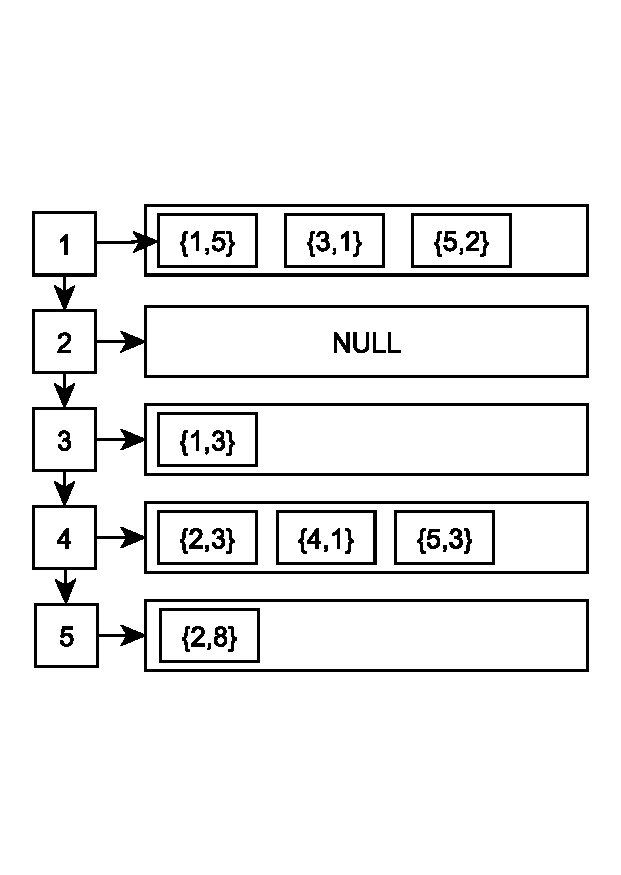
\includegraphics[width=0.5\textwidth, trim = 0mm 33mm 0mm 33mm, clip]{file_processing.pdf}
\caption{Struktura zapisana w pliku}
\label{fig:preprocessing_fig}
\end{figure}

Wynikiem działania tej części preprocesingu jest struktura będąca HashMapą. Zawierająca ona w komórce $i$ listę wszystkich niezerowych elementów znajdujących się w i-tym wierszu macierzy wraz z ich wartościami. Figura \ref{fig:preprocessing_fig} pokazuje fragment macierzy, który zostanie zapisany do pliku. Poniżej znajduje sie macierz $M_{5,5}$, która powstanie ze struktury przedstawionej na \ref{fig:preprocessing_fig}


\[
 M_{5,5} =
 \begin{pmatrix}
5 & 0 & 1 & 0 & 2\\
0 & 0 & 0 & 0 & 0\\
3 & 0 & 0 & 0 & 0\\
0 & 3 & 0 & 1 & 3\\
0 & 8 & 0 & 0 & 0\\

 \end{pmatrix}
\]


\subsection{Inne metody przyśpieszenia wykonywanych preprocesingów}

Jednym z głównym problemów jest to, że w czasie wykonywania wymienionych powyżej procedur, tabele USER, TAG i DOCUMENT są zablokowane na zmiany. W działającej aplikacji byłoby to poważnym problemem.  

Można poradzić sobie z tym problemem poprzez posiadanie kopi bazy danych i uzupełnianie obydwu jednocześnie. Dzięki czemu operacje wymagające dużej ilości czasu, mogłyby być wykonane na innej bazie. Po dokonaniu wszystkich obliczeń wymagane jest zsynchronizowanie obydwu baz danych.

Inną możliwością jest zrównoleglenie wykonywanych obliczeń. Możliwe jest na przykład: podzielenie obliczenia tabel TAG\_DOC, TAG\_USER i USERTAGDOC na różne maszyny. Dodatkową możliwością jest podzielenie samych tabel na różne procesy. Na przykład wyliczanie tabeli TAG\_DOC można podzielić na niezależne procesy ze względu na pole ID obiektów z tabeli TAG. Analogicznie można przeprowadzić taki podział dla innych tabel.

Kolejną możliwością są zmiany danych w tabelach TAG\_DOC, TAG\_USER i USERTAGDOC w czasie kiedy dodawane są nowe rekordy do tabel USER, DOCUMENT i TAG. Wyeliminowało by to potrzebę wykonywania opisane powyżej preprocesingu, ale stanowiło by problem przy tworzeniu macierzy. Tworzenie macierzy (dokładnie: plików z których następnie tworzona jest macierz) jest czasochłonne i wymaga zatrzymania zmian dokonywanych na tabelach TAG\_DOC, TAG\_USER i USERTAGDOC. Problem ten dałoby się rozwiązać przez np: posiadanie kopi wymienionych wcześniej tabel. Synchronizacja kopi tabeli i głównej tabeli nie zajmowała by aż tak wiele czasu. Pomysł ten spowodował by jeszcze jeden potencjalnie groźny problem. Ilość operacji, które trzeba by wykonać w czasie gdy dodawane są nowe rekordy do tabel, znacznie by się zwiększyła. Mogłoby to spowodować większą awaryjność np: problemy z transakcjami.














\section{Tworzenie macierzy na potrzeby algorytmów}
W algorytmach Social PageRank i Adapted PageRank potrzebne są 3 rodzaje macierzy i ich transpozycje. Macierze te są tworzone z danych zebranych z serwisu delicous:
\begin{itemize}
	\item $M_{UT}$ macierz ta zawiera w komórce $m_{n,m}$ informacje o ilości dokumentów dodanych przez użytkownika $u_n$ i opisanych tagiem $t_m$. Dane, z których zostaje utworzona ta macierz znajdują się w tabeli TAG\_USR. Tabela ta została wyliczona w czasie preprocessingu.
	\item $M_{TD}$ macierz ta zawiera w komórce $m_{n,m}$ informacje o ilości użytkowników którzy opisali tagiem $t_n$ dokument $d_m$. Źródłem danych dla taj macierzy jest tabela TAG\_DOC
	\item $M_{DU}$ analogicznie, ta macierz zawiera dane na temat ilości tagów. Informacje pobierane są z tabeli USERTAGDOC
\end{itemize}

Wykorzystywane są one w kolejnych iteracjach algorytmu Social PageRank. Przy algorytmie Adapted PageRank są one używane pośrednio. Struktura na której operuje algorytm Adapted pagerank jest macierzą złozoną z macierzy $M_{UD} , M_{TD}, M_{UT}$ i ich transpozycji. Macierzy używana w algorytmie wygląda następująco:

\[
 G_f =
 \begin{pmatrix}
  0                     & M_{DU}       & M_{TD}^T \\
  M_{DU}^T  & 0                     & M_{UT}     \\
  M_{TD}       & M_{UT}^T   & 0 
 \end{pmatrix}
\]

Ważną cechą macierzy na których przeprowadzane są operacje jest to, że są to macierze rzadkie. Liczba niezerowych komórek w macierzy wynosi:  [TODO, dane się zmieniły, uzupełnić po testach]

\section{Operacje przeprowadzane na macierzach}
W każdej iteracji algorytmów, główna operacją przeprowadzaną jest mnożenie wymienionych wcześniej macierzy przez wektor. Operacja ta jest przeprowadzana do czasu uzyskania zbieżności wartości wektora wynikowego.

Z powodu wielkości macierzy w aplikacji nie możemy wczytać bezpośrednio całych macierzy do pamięci i na nich operować. Dodatkowo używana biblioteka stawia ograniczenie na iloczyn kolumn i wierszy takie że: $ilosc\_kolumn * ilosc\_wierszy <= 2^{31}-1$.  Gdzie wartość $2^{31}-1$ jest to maksymalna liczba jaką można przypisać zmiennej typu integer w języku Java. 



\subsection*{Implementacja}

\begin{figure}[htb]
\centering
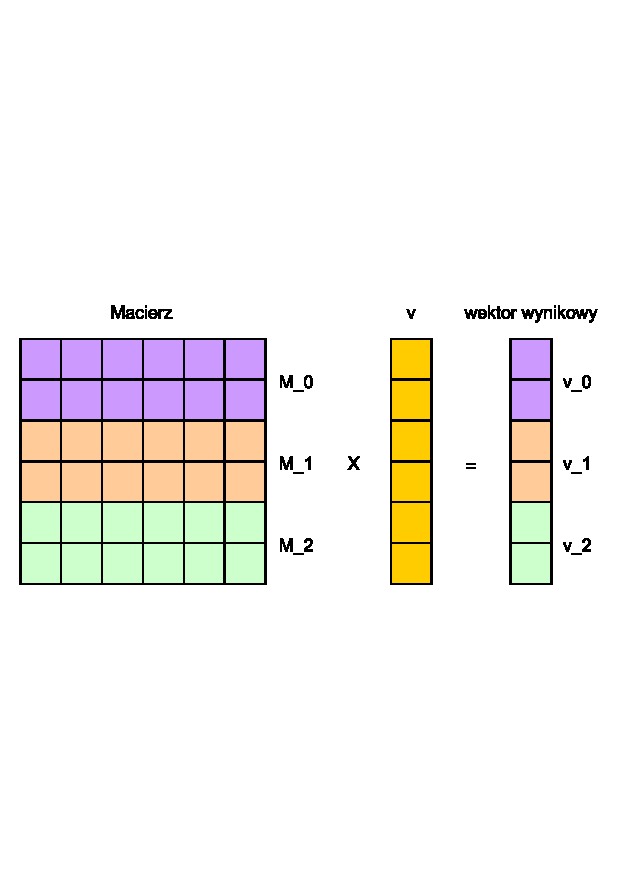
\includegraphics[width=1\textwidth, trim = 0mm 45mm 0mm 50mm, clip]{matrix_multiply.pdf}
\caption{Mnożenie macierzy przez wektor v}
\label{fig:matrix_mult_fig}
\end{figure}

Mnożenie macierzy odbywa się częściami. Bierzemy fragment macierzy: $M_{i}$ i mnożymy go przez wektor $v$. Wynikiem jest wektor $p_i$, który stanowi i-ty fragment wynikowego wektora. Powstałe fragmenty wektora łączymy razem w odpowiedniej kolejności otrzymując w ten sposób w wektor wynikowy (\ref{fig:matrix_mult_fig})




\lstset{language=Python}
\begin{lstlisting}[frame=lines, caption={Mnożenie macierzy przez wektor v}, label={list:matrix_mult_fig}] ]
def matrix_multiply(v, matrix_source):
	v_return = empty_vector()  #wektor zwracany
	for matrix_part in matrix_source.get_part_matrixes():
		#mnozenie macierzy i wektora
		v_part = multiply(matrix_part, v) 
		# dokladamy wyliczony fragment wektora na koniec
		v_return.append(v_part)   
	return v_return 
\end{lstlisting}

Mnożenie odbywa się poprzez funkcje z biblioteki Colt. Biblioteka ta uwzględnia to, że macierz na której odbywają się operacje jest macierzą rzadką. Oszczędzana jest pamięć przez zapisywanie tylko niezerowych elementów. W czasie mnożenia przez wektor pomijane są wszystkie zerowe komórki, przez co sama operacja mnożenia jest krótka. Najwięcej czasu zajmuje samo tworzenie częściowych  macierzy i ładowanie plików zawierających kolejne fragmenty macierzy. 


\subsection{Inne metody przyśpieszenia obliczeń na macierzach}

Opisana powyżej metoda nie mogłaby zostać wykorzystana w działającej. Przy tylko 1 milionie dokumentów czas wykonania algorytmu Social PageRank wynosi około 36 godzin[FIXME, inne dane, inne czasy]. Prawdziwy system zawierałby zdecydowanie więcej danych. Poniżej opisanych jest kilka  pomysłów na ulepszenie i przyśpieszenie działania aplikacji

\subsection*{Zmiana języka w którym została zaimplementowana aplikacja}
Maszyna wirtualna Javy nie jest bardzo wydajna jeśli chodzi o szybkość obliczeń, dodatkowo dochodzą ograniczenia związane np: z pamięcią. Możliwe jest również przepisanie tylko kluczowych dla obliczeń fragmentów, a następnie ich uruchamianie z aplikacji. 

\subsection*{Proste zrównoleglenie obliczeń}
Wykorzystując opisaną wcześniej metodę dzielenia macierzy na kawałki, możliwe jest podzielenie macierzy na różne procesory/maszyny. Każdy proces po zakończeniu obliczania swojej części zapisałby wynikowy wektor do np: bazy danych, w której następowałaby synchronizacja procesów. 

\subsection*{Obliczanie przy użyciu GPU/CUDA} 

Możliwe jest wykorzystanie GPU do wykonania obliczeń na macierzach. Obecne jednostki graficzne zawierają dodatkowe technologie wspomagające operacje na macierzach rzadkich. 

\subsection*{Wykorzystanie innych aplikacji}

Obliczanie kolejnych iteracji mogłoby również być przerzucone na zewnętrzną aplikacji np: MATLAB.





\chapter{Dane [TODO]}

[ statystyki danych, czyszczenie danych, wyszukiwanie outlierów, ... ]
\chapter{Wyniki [TODO]}

TODO

\bibliographystyle{plain}
\bibliography{biblio}


\end{document}
